% !TEX root = ../tex/7-5.tex
% 第7章：本文は青、補足は緑
\newcommand{\asmain}{%
    \setbeamercolor{frametitle}{fg=white,bg=main}%
    \setbeamercolor{structure}{fg=main}%
    \setbeamercolor{itemize item}{fg=main}%
    \setbeamercolor{itemize subitem}{fg=main}%
    \setbeamercolor{enumerate item}{fg=main}%
}
\newcommand{\assuppl}{%
    \setbeamercolor{frametitle}{fg=white,bg=examplecol}%
    \setbeamercolor{structure}{fg=examplecol}%
    \setbeamercolor{itemize item}{fg=examplecol}%
    \setbeamercolor{itemize subitem}{fg=examplecol}%
    \setbeamercolor{enumerate item}{fg=examplecol}%
}
\newcommand{\supplmark}{%
    \setlength{\fboxsep}{1.5pt}%
    \setlength{\fboxrule}{0.7pt}%
    \fbox{\textbf{補足}}%
}
\asmain


%=============================================
\begin{frame}{7.5 Is Diffusion Model's ODE an Optimal Map?}
    \begin{block}{この節の問い（論文 7.5）}
        拡散の PF-ODE が誘導する決定的フロー写像は、\\
        二次コストの最適輸送（OT）マップと一致するか？
    \end{block}
    \begin{itemize}
        \item 対象は二次コスト OT（$W_2$ / Benamou--Brenier）
        \item 答えは一般に\textbf{No}（反例と構造的議論がある）
        \item 線形流・Reflow も、OT ソルバとしては保証が弱い
    \end{itemize}
\end{frame}
%=============================================
\asmain
\begin{frame}{7.5 の道筋}
    \begin{enumerate}
        \item \textbf{7.5.1 PF-ODE は一般に OT ではない}\\
        ガウス設定の反例、Lavenant--Santambrogio、Brenier（Thm.\ 7.1）
        \item \textbf{7.5.2 線形流と Reflow}\\
        条件付き流による運動エネルギー上界（Prop.\ 7.5.1）\\
        Rectify / Reflow の固定点 $\neq$ OT（反例）
        \item \textbf{Takeaway}\\
        いつ一致し、いつ一致しないか
    \end{enumerate}
\end{frame}
%=============================================
\asmain
\begin{frame}{前回までとの接続}
    \begin{itemize}
        \item \textbf{7.2--7.3}：静的 OT / 動的 Benamou--Brenier / EOT / SB
        \item \textbf{7.4}：標準的な拡散 SDE は、一般に指定端点の SB を解かない
        \item \textbf{ここ（7.5）}：ODE 側 --- PF-ODE は決定的輸送マップを定めるが、\\
        二次コスト OT の最小化子とは限らない
    \end{itemize}
    \begin{exampleblock}{生成設定}
        典型的には $p_{\mathrm{src}}=p_{\mathrm{prior}}$（ガウス）、$p_{\mathrm{tgt}}=p_{\mathrm{data}}$。\\
        議論では $p_0\to\mathcal{N}(0,I)$ 向きでも同じ問いになる。
    \end{exampleblock}
\end{frame}
%=============================================
\section{7.5.1 PF-ODE Is Generally Not OT}
\asmain
\begin{frame}{区切り：7.5.1 PF-ODE は一般に OT ではない}
    \tableofcontents[currentsection]
\end{frame}
%=============================================
\asmain
\begin{frame}{自然な問い}
    \begin{block}{Question}
        拡散過程が誘導する決定的フロー写像は、\\
        二次コストの OT マップと一致するか？
    \end{block}
    \begin{alertblock}{答え}
        \textbf{一般には No。}\\
        端点分布がガウスでも、明示的な反例がある\\
        （例：Tanana 2017；より強い構成は Lavenant \& Santambrogio 2022）。
    \end{alertblock}
\end{frame}
%=============================================
\asmain
\begin{frame}{Figure 7.6：PF-ODE と OT マップは見た目も違う}
    \centering
    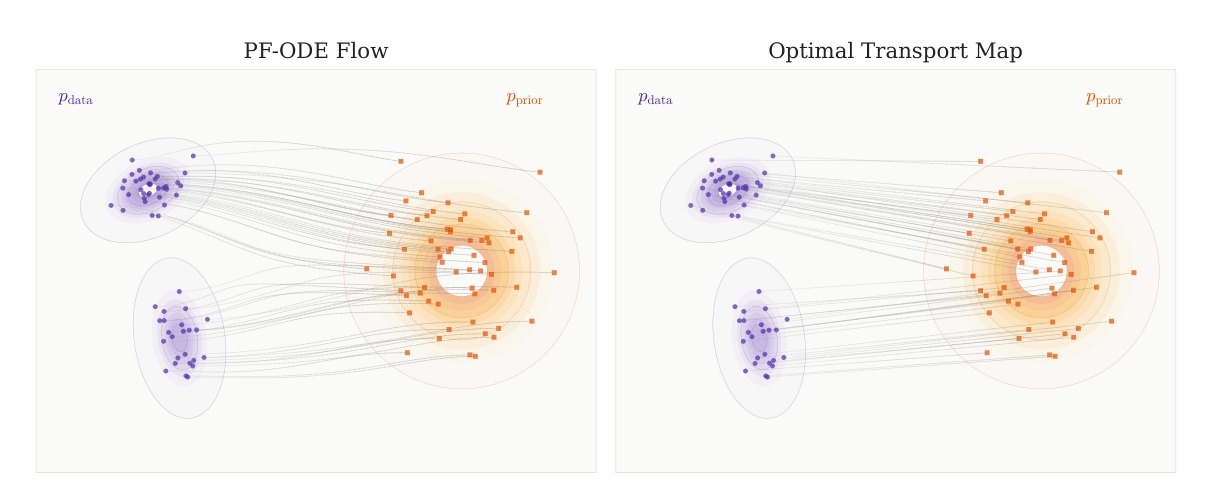
\includegraphics[width=\textwidth,height=0.62\textheight,keepaspectratio]{fig-7-6.jpg}
    \vfill
    \footnotesize
    左：PF-ODE を積分したフロー写像。右：Hungarian で得た二次コスト OT。\\
    同じ端点でも対応（および軌道）が異なり、PF-ODE $\neq$ OT を直感的に示す。\\
    Source: Created by the authors with AI-assisted coding.
\end{frame}
%=============================================
\asmain
\begin{frame}{図の読み方}
    \begin{columns}[T,onlytextwidth]
        \begin{column}{0.48\textwidth}
            \begin{block}{左：PF-ODE}
                周辺密度を運ぶ確率流の積分。\\
                端点周辺は合っていても、\\
                点の対応は OT とは限らない。
            \end{block}
        \end{column}
        \begin{column}{0.48\textwidth}
            \begin{block}{右：OT マップ}
                二次コストを最小にする対応\\
                （Brenier マップ）。\\
                直線補間が変位補間になる。
            \end{block}
        \end{column}
    \end{columns}
    \begin{exampleblock}{要点}
        「同じ周辺を結ぶ」ことと「二次コスト最適」は別の要求である。
    \end{exampleblock}
\end{frame}
%=============================================
\asmain
\begin{frame}{Setup：OU（VP）と PF-ODE}
    初期密度 $p_0$ を標準ガウスへ運ぶ Ornstein--Uhlenbeck：
    \[
        \mathrm{d}x(t)=-x(t)\,\mathrm{d}t+\sqrt{2}\,\mathrm{d}w(t),\qquad
        x(0)\sim p_0.
    \]
    対応する PF-ODE（フロー写像 $S_t$）：
    \[
        \frac{\mathrm{d}S_t(x)}{\mathrm{d}t}
        =
        -S_t(x)-\nabla\log p_t\!\bigl(S_t(x)\bigr),\qquad
        S_0(x)=x.
    \]
    \begin{itemize}
        \item $(S_t)_{\#}p_0=p_t$
        \item 速度 $v_t(x)=-x-\nabla\log p_t(x)$
        \item $t\to\infty$ で $S_\infty\#p_0=\mathcal{N}(0,I)=:p_{\mathrm{prior}}$
    \end{itemize}
\end{frame}
%=============================================
\asmain
\begin{frame}{Fokker--Planck と連続の式}
    周辺 $p_t$ は
    \[
        \partial_t p_t=\nabla\cdot(x\,p_t)+\Delta p_t
    \]
    に従う。これは速度 $v_t(x)=-x-\nabla\log p_t(x)$ の連続の式と同値：
    \[
        \partial_t p_t+\nabla\cdot(p_t v_t)=0,\qquad
        \frac{\mathrm{d}S_t}{\mathrm{d}t}=v_t(S_t).
    \]
    \begin{block}{意味}
        PF-ODE は「正しい周辺経路を運ぶ決定的力学」を与える。\\
        しかし、その力学が Benamou--Brenier の最小化子であるとは限らない。
    \end{block}
\end{frame}
%=============================================
\asmain
\begin{frame}{Lavenant--Santambrogio の狙い}
    彼らは単に「終端マップ $S_\infty:p_0\to\mathcal{N}(0,I)$ が最適か」だけを見ない。\\
    代わりに、\textbf{フロー全体}を調べる。
    \[
        T_{t\to\infty}:=S_\infty\circ S_t^{-1}
    \]
    は、中間周辺 $p_t$ からガウスへの残差輸送マップ。
    \begin{alertblock}{主張の核}
        上手く選んだ $p_0$ に対し、ある $t_0\ge 0$ で\\
        $T_{t_0\to\infty}$ が $p_{t_0}\to\mathcal{N}(0,I)$ の二次コスト OT にならない。
    \end{alertblock}
    \footnotesize
    したがって「PF-ODE 流はずっと OT」という性質は、一般には成り立たない。
\end{frame}
%=============================================
\assuppl
\begin{frame}{\supplmark：なぜ「途中で壊れる」を見るのか}
    \begin{itemize}
        \item 終端だけ最適でも、中間から見た残差が最適とは限らない
        \item OT の動的定式化では、経路全体の運動エネルギーを見る
        \item 「全時刻で OT」を仮定すると強い必要条件が出る（後述の交換条件）
        \item その必要条件を破る $p_0$ を作れば、反例になる
    \end{itemize}
    \begin{exampleblock}{メッセージ}
        非最適性は、端点の偶然一致ではなく、フローの構造に根ざす。
    \end{exampleblock}
\end{frame}
%=============================================
\asmain
\begin{frame}{Theorem 7.1（Informal Brenier's Theorem）}
    滑らかな密度をもつ確率分布 $\nu_1,\nu_2$ について、\\
    滑らかな写像 $T$ が二次コスト OT であることと、\\
    ある凸関数 $u$ について $T=\nabla u$ であることは同値。
    \begin{itemize}
        \item このとき $DT$ は対称かつ半正定値
        \item $u$ は Monge--Amp\`ere を満たす：
        \[
            \det D^2 u(x)
            =
            \frac{\nu_1(x)}{\nu_2(\nabla u(x))}
        \]
    \end{itemize}
    \vfill
    \footnotesize
    補足：写像が OT なら、その逆写像は逆向きの OT である。
\end{frame}
%=============================================
\asmain
\begin{frame}{証明スケッチ：仮定（背理法）}
    すべての $t\ge 0$ で
    \[
        T_t:=S_t\circ S_\infty^{-1}
    \]
    が $\mathcal{N}(0,I)\to p_t$ の二次コスト OT だと仮定する。
    \begin{enumerate}
        \item Brenier $\Rightarrow$ $DT_t$ は常に対称（かつ半正定値）
        \item 対称性を時間微分し、フローの線形化と合わせる
        \item $t=0$ で「Hessian と Jacobian の交換」必要条件を得る
        \item その条件を破る凸ポテンシャル $u$ を作り、矛盾を得る
    \end{enumerate}
\end{frame}
%=============================================
\assuppl
\begin{frame}{\supplmark：Step 1--2（対称性の伝播）}
    Brenier より $DT_t(x)$ は対称。時間微分も対称を保つ。
    \[
        \partial_t(DS_t)=Dv_t(S_t)\,DS_t
        =\bigl(-I-D^2\log p_t(S_t)\bigr)DS_t.
    \]
    これを $DT_t=DS_t(S_\infty^{-1})\,D(S_\infty^{-1})$ に代入すると、\\
    特に $t=0$（$S_0=I$）で
    \[
        \bigl(-I-D^2\log p_0(S_\infty^{-1}(x))\bigr)\,D(S_\infty^{-1})(x)
    \]
    が対称でなければならない。
\end{frame}
%=============================================
\assuppl
\begin{frame}{\supplmark：Step 3（交換条件）}
    $T_0=S_\infty^{-1}$ も OT なら $D(S_\infty^{-1})$ は対称。\\
    $D^2\log p_0$ も対称。\\
    対称行列の積が対称 $\Leftrightarrow$ 両者が交換する。よって
    \[
        D^2\log p_0(y)
        \quad\text{が}\quad
        DS_\infty(y)
        \quad\text{と交換}
        \qquad(\forall y).
    \]
    $S_\infty=\nabla u$（凸）と Monge--Amp\`ere から
    \[
        D^2\!\left(\log\det D^2 u-\tfrac12\|\nabla u\|^2\right)
        \quad\text{が}\quad
        D^2 u
        \quad\text{と交換}
        \tag{7.5.1}
    \]
    が必要。
\end{frame}
%=============================================
\assuppl
\begin{frame}{\supplmark：Step 4（反例の構成）}
    \[
        u(x)=\tfrac12\|x\|^2+\varepsilon\,\phi(x)
        \quad(\varepsilon\text{ 小})
    \]
    とおくと、$x=0$ での交換条件は概ね
    「$D^2\phi(0)$ が $D^2(\Delta\phi)(0)$ と交換」を要求する。
    \begin{exampleblock}{$\mathbb{R}^2$ の例}
        $\phi(x_1,x_2)=x_1 x_2+x_1^4$ は交換条件を破る。\\
        $p_0=(\nabla u)^{-1}\#\mathcal{N}(0,I)$ とすれば、$S_\infty=\nabla u$ は端点 OT だが、\\
        「全時刻 OT」仮定は破綻する。
    \end{exampleblock}
    よってある $t_0$ で $T_{t_0\to\infty}$ は OT ではない。
\end{frame}
%=============================================
\asmain
\begin{frame}{7.5.1 の結論}
    \begin{itemize}
        \item PF-ODE は周辺を正しく運ぶ決定的マップを与える
        \item しかし二次コスト OT（Brenier）とは一般に一致しない
        \item ガウス端点でも、明示的・構造的な反例がある
        \item 「端点が正しい」$\neq$「コスト最適」
    \end{itemize}
    \begin{alertblock}{標語}
        PF-ODE は admissible な決定的カップリングの一つであり、\\
        Benamou--Brenier 作用の最小化子ではない（一般に）。
    \end{alertblock}
\end{frame}
%=============================================
\section{7.5.2 Canonical Linear Flow and Reflow}
\asmain
\begin{frame}{区切り：7.5.2 線形流と Reflow は OT に至るか}
    \tableofcontents[currentsection]
\end{frame}
%=============================================
\asmain
\begin{frame}{次の自然な問い}
    PF-ODE（特に VP 型）は一般に OT ではない。では：
    \begin{block}{Question 7.5.1}
        独立カップリング $\pi(x_0,x_1)=p_{\mathrm{src}}(x_0)p_{\mathrm{tgt}}(x_1)$ の下で、\\
        線形補間流 $(1-t)x_0+t x_1$ は OT マップを回復するか？
    \end{block}
    \begin{alertblock}{答え}
        \textbf{No。}\\
        ただし、線形経路は「与えられたカップリングに対する」\\
        運動エネルギー上界のうち最良を与える（Prop.\ 7.5.1）。
    \end{alertblock}
\end{frame}
%=============================================
\asmain
\begin{frame}{復習：Benamou--Brenier（動的 OT）}
    二次コスト OT の動的形（論文 (7.2.3)）：
    \[
        \mathcal{K}(p_{\mathrm{src}},p_{\mathrm{tgt}})
        :=
        \min_{(p_t,v_t)}
        \int_0^1\!\!\int_{\mathbb{R}^D}
        \|v_t(x)\|^2\,p_t(x)\,\mathrm{d}x\,\mathrm{d}t
    \]
    拘束：$\partial_t p_t+\nabla\cdot(p_t v_t)=0$、$p_0=p_{\mathrm{src}}$、$p_1=p_{\mathrm{tgt}}$。
    \begin{itemize}
        \item 静的 Monge は Monge--Amp\`ere を解く必要がある
        \item 動的形は凸再定式化できるが、高次元グリッドでは依然困難
    \end{itemize}
\end{frame}
%=============================================
\asmain
\begin{frame}{条件付き流による上界の発想}
    真の $\mathcal{K}$ を直接解く代わりに、\\
    固定端点 $(x_0,x_1)\sim\pi_{0,1}$ をつなぐ条件付き経路族に制限する。
    \begin{itemize}
        \item 任意の条件付き流 $\Psi_t(x_0,x_1)$ の経路エネルギー期待値が上界
        \item その族の中で最良の経路形状を選ぶと線形補間になる
        \item Flow Matching / Rectified Flow の前向き核と一致
    \end{itemize}
    \begin{exampleblock}{注意}
        条件付き族での最適 $\neq$ 周辺に対する大域最適。
    \end{exampleblock}
\end{frame}
%=============================================
\asmain
\begin{frame}{Proposition 7.5.1：運動エネルギーの上界}
    任意のカップリング $\pi_{0,1}$ について：
    \begin{enumerate}
        \item 任意の条件付き流 $\Psi_t$ に対し
        \[
            \mathcal{K}(p_{\mathrm{src}},p_{\mathrm{tgt}})
            \le
            \mathbb{E}_{(x_0,x_1)\sim\pi_{0,1}}
            \!\left[\int_0^1\|\Psi_t'(x_0,x_1)\|^2\,\mathrm{d}t\right]
        \]
        \item 右辺を最小にする一意な条件付き流は線形補間
        \[
            \Psi_t^\star(x_0,x_1)=(1-t)x_0+t x_1
        \]
        であり、最良上界は
        \[
            \mathcal{K}\le\mathbb{E}_{(x_0,x_1)\sim\pi_{0,1}}\|x_1-x_0\|^2
        \]
    \end{enumerate}
\end{frame}
%=============================================
\assuppl
\begin{frame}{\supplmark：Prop.\ 7.5.1 の証明の骨子}
    \begin{itemize}
        \item Jensen と条件付き期待値の塔法則で、\\
        周辺運動エネルギー $\le$ 条件付き経路エネルギーの期待値
        \item 端点固定の変分問題を Euler--Lagrange で解くと直線が最適
        \item 詳細は Lipman et al.\ (2024) §4.7
    \end{itemize}
    \begin{block}{読み方}
        線形 FM / RF 経路は「与えられたペアリングに対する最良上界」を与える。\\
        ペアリング自体が悪いと、上界は真の OT コストから遠くなりうる。
    \end{block}
\end{frame}
%=============================================
\asmain
\begin{frame}{独立カップリング＋直線は OT ではない}
    もっとも素朴な計画：独立サンプルを直線で結ぶ。
    \begin{itemize}
        \item 失敗の主因は「直線であること」ではない
        \item \textbf{点の結び方（カップリング）が非効率}なこと
        \item Prop.\ 7.5.1 は、悪い $\pi$ の下でも直線が上界を最良化する、と言うだけ
    \end{itemize}
    \begin{exampleblock}{5.4 との接続}
        直線化は二次コスト OT の必要条件だが十分条件ではない\\
        （5.4 の予告どおり。ここがその本編）。
    \end{exampleblock}
\end{frame}
%=============================================
\asmain
\begin{frame}{Reflow は建設的な応答か？}
    Reflow はペアリングを直す反復手続き（§5.4）。
    \[
        \pi^{(k+1)}=\mathrm{Rectify}(\pi^{(k)}),\qquad
        \pi^{(0)}=p_{\mathrm{src}}\,p_{\mathrm{tgt}}
    \]
    \begin{itemize}
        \item 各ステップで輸送コストは非増加（Liu, Gong et al., 2022）
        \item より良い配置へ押しやる、という直感はある
        \item では固定点／極限は OT か？
    \end{itemize}
\end{frame}
%=============================================
\asmain
\begin{frame}{Question 7.5.2}
    \begin{block}{問い}
        Rectify を反復すると、輸送計画は OT に収束するか？\\
        Reflow の固定点は OT マップを与えるか？
    \end{block}
    \begin{alertblock}{短い答え}
        \textbf{一般には No。}
    \end{alertblock}
    以下、何が壊れうるかを整理する。
\end{frame}
%=============================================
\asmain
\begin{frame}{Rectify 反復の中身}
    各 $k$ で速度場を（非パラメトリックに）
    \[
        v_t^{(k)}\in\argmin_{u_t}\,L(u_t\mid\pi^{(k)})
    \]
    と学び、積分マップ $\Psi_1^{(k)}$ で
    \[
        \pi^{(k+1)}(x_0,x_1)
        =
        p_{\mathrm{src}}(x_0)\,
        \delta\!\bigl(x_1-\Psi_1^{(k)}(x_0)\bigr)
    \]
    と更新する。
    \begin{itemize}
        \item $L=0$ を達成する $v_t$ があっても、輸送が OT とは限らない\\
        （Liu, Gong et al., 2022 の観察）
        \item 直線化・損失ゼロは最適性の十分条件ではない
    \end{itemize}
\end{frame}
%=============================================
\asmain
\begin{frame}{ポテンシャル拘束：$\mathrm{Rectify}^\perp$}
    Benamou--Brenier の最適速度はポテンシャル場（勾配場）。\\
    そこで損失を勾配場に制限する提案（Liu 2022）：
    \[
        w_t^{(k)}\in
        \argmin_{u_t=\nabla\phi}\,L(u_t\mid\pi^{(k)})
        \tag{7.5.2}
    \]
    この演算子を $\mathrm{Rectify}^\perp$ と書く（非回転成分への射影の意味）。
    \begin{exampleblock}{ねらい}
        「損失ゼロ＋勾配場」なら OT、という特徴づけを期待する。
    \end{exampleblock}
\end{frame}
%=============================================
\asmain
\begin{frame}{予想された同値（しかし反例あり）}
    カップリング $\pi$ について、次の同値が予想された：
    \begin{enumerate}
        \item[(i)] $\pi$ は OT カップリング
        \item[(ii)] $\pi=\mathrm{Rectify}^\perp(\pi)$（固定点）
        \item[(iii)] ある勾配速度 $v_t=\nabla\phi_t$ で $L(v_t\mid\pi)=0$
    \end{enumerate}
    \begin{alertblock}{Hertrich et al.\ (2025)}
        この同値は一般には成り立たない（二種類の反例）。
    \end{alertblock}
\end{frame}
%=============================================
\assuppl
\begin{frame}{\supplmark：反例の二類型}
    \begin{enumerate}
        \item \textbf{非連結サポート}\\
        中間分布 $p_t$ が非連結だと、\\
        $\mathrm{Rectify}^\perp$ の固定点・損失ゼロ・勾配場でも\\
        最適カップリングにならない例がある
        \item \textbf{ガウス端点でも}\\
        損失を任意に小さくできても、\\
        最適カップリングからのずれを任意に大きくできる例がある
    \end{enumerate}
    \begin{exampleblock}{含意}
        Rectified Flow は強い生成モデルになりうるが、\\
        原理的な OT ソルバとしての信頼性は限定的。
    \end{exampleblock}
\end{frame}
%=============================================
\asmain
\begin{frame}{生成性能と輸送コストは別物}
    \begin{itemize}
        \item 輸送コストが下流タスク性能と常に相関するわけではない
        \item 厳密な OT マップの計算が、必ずしも実務上の最良結果を生まない
        \item それでも OT / EOT / SB の変種は科学・工学で基本的
        \item 拡散モデルは、その探索のための強力な枠組みを提供する
    \end{itemize}
\end{frame}
%=============================================
\section{Takeaway}
\asmain
\begin{frame}{区切り：いつ一致し、いつ一致しないか}
    \tableofcontents[currentsection]
\end{frame}
%=============================================
\asmain
\begin{frame}{Takeaway：ODE と OT}
    \renewcommand{\arraystretch}{1.25}
    \begin{tabular}{p{0.42\textwidth}p{0.48\textwidth}}
        \textbf{一致／近い場合のイメージ} &
        \textbf{一致しない典型} \\
        \hline
        1次元の単調再配列など、\\
        構造が強い特殊設定 &
        一般の多次元 PF-ODE 流 \\
        勾配場＋真の OT カップリング &
        独立カップリング＋線形 FM \\
        （理論上の Brenier マップ） &
        Reflow 固定点（一般） \\
    \end{tabular}
    \vfill
    \begin{block}{一文}
        拡散 ODE は決定的輸送を与えるが、二次コスト OT そのものではない。\\
        線形化・Reflow は上界改善・直線化の道具であり、OT 求解の保証ではない。
    \end{block}
\end{frame}
%=============================================
\asmain
\begin{frame}{チェックリスト（7.5）}
    \begin{itemize}
        \item PF-ODE は周辺を運ぶが、Brenier マップとは限らない
        \item Fig.\ 7.6：同じ端点でも対応が目に見えて違う
        \item Thm.\ 7.1：OT $\Leftrightarrow$ 凸ポテンシャルの勾配
        \item Prop.\ 7.5.1：線形条件付き流は運動エネルギー上界を最良化
        \item Q7.5.1 / Q7.5.2：独立線形流も Reflow も、一般に OT ではない
        \item 生成モデルとしての有用性と、OT ソルバとしての厳密性は切り分ける
    \end{itemize}
\end{frame}
%=============================================
\asmain
\begin{frame}{7.5 のまとめ}
    \begin{itemize}
        \item 二次コスト OT に対し、PF-ODE 流は一般に最適ではない
        \item Lavenant--Santambrogio は「全時刻 OT」仮定の破綻を示す
        \item 線形 FM 経路は与えられたカップリングに対する最良上界を与える
        \item Reflow / $\mathrm{Rectify}^\perp$ にも OT 収束の一般保証はない
        \item 次節 7.6：章全体の総括と、決定的輸送の広い風景
    \end{itemize}
\end{frame}
